\documentclass[tikz,border=10pt]{standalone}
\usepackage{tikz}
\usetikzlibrary{positioning, fit, arrows.meta, calc, shapes.geometric}

\begin{document}

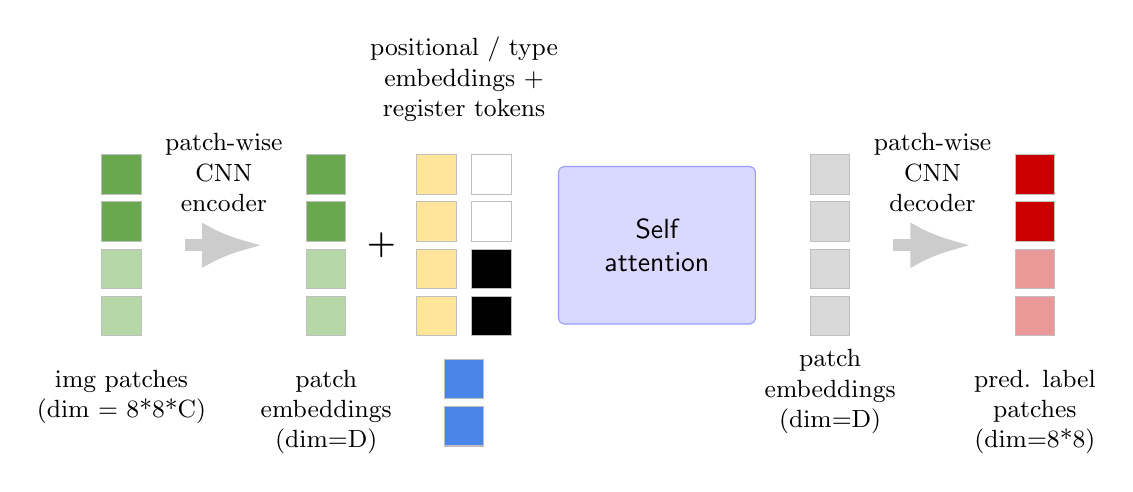
\begin{tikzpicture}[
    font=\sffamily,
    >=LaTeX,
    node distance=0.5cm,
    % --- Styles ---
    patch/.style={draw=gray!50, thin, minimum size=0.5cm, inner sep=0pt, anchor=center},
    block/.style={draw=blue!40, fill=blue!15, minimum width=2.5cm, minimum height=2.0cm, rounded corners=2pt, align=center},
    arrow_gray/.style={->, line width=1.5mm, color=black!20},
    label_text/.style={align=center, font=\small, color=black},
    plus/.style={font=\large\bfseries, text=black}
]

    % --- Colors (Matched to previous diagrams) ---
    \definecolor{tGreen}{RGB}{106,168,79}   % Target Green
    \definecolor{cGreen}{RGB}{182,215,168}  % Context Green
    \definecolor{tRed}{RGB}{204,0,0}        % Target Red
    \definecolor{cRed}{RGB}{234,153,153}    % Context Red
    \definecolor{pYellow}{RGB}{255,229,153} % Positional Yellow
    \definecolor{typeBlack}{RGB}{0,0,0}     % Type Black
    \definecolor{regBlue}{RGB}{74,134,232}  % Register Token Blue
    \definecolor{embGrey}{RGB}{217,217,217} % Embedding Grey

    % ==========================
    % 1. INPUT: IMG PATCHES
    % ==========================
    \coordinate (start) at (0,0);
    
    % Stack 1: Input Images
    \node[patch, fill=tGreen] (i1) at (0, 2.4) {};
    \node[patch, fill=tGreen] (i2) at (0, 1.8) {};
    \node[patch, fill=cGreen] (i3) at (0, 1.2) {};
    \node[patch, fill=cGreen] (i4) at (0, 0.6) {};
    
    \node[label_text, below=0.3cm of i4] {img patches\\(dim = 8*8*C)};

    % Arrow: Encoder
    \draw[arrow_gray] (0.8, 1.5) -- (1.8, 1.5);
    \node[label_text, above=0.3cm] at (1.3, 1.5) {patch-wise\\CNN\\encoder};


    % ==========================
    % 2. PATCH EMBEDDINGS
    % ==========================
    
    % Stack 2: Green Embeddings
    \coordinate (emb_col) at (2.6, 0);
    \node[patch, fill=tGreen] (e1) at (2.6, 2.4) {};
    \node[patch, fill=tGreen] (e2) at (2.6, 1.8) {};
    \node[patch, fill=cGreen] (e3) at (2.6, 1.2) {};
    \node[patch, fill=cGreen] (e4) at (2.6, 0.6) {};

    \node[label_text, below=0.3cm of e4] {patch\\embeddings\\(dim=D)};

    % Plus Sign
    \node[plus] at (3.3, 1.5) {+};


    % ==========================
    % 3. POSITIONAL / TYPE / REGISTERS
    % ==========================
    
    % Column 1: Positional (Yellow)
    \coordinate (pos_col) at (4.0, 0);
    \foreach \y in {2.4, 1.8, 1.2, 0.6} {
        \node[patch, fill=pYellow] at (4.0, \y) {};
    }

    % Column 2: Type (White/Black)
    \coordinate (type_col) at (4.7, 0);
    \node[patch, fill=white, draw=gray!50] at (4.7, 2.4) {};
    \node[patch, fill=white, draw=gray!50] at (4.7, 1.8) {};
    \node[patch, fill=typeBlack] at (4.7, 1.2) {};
    \node[patch, fill=typeBlack] at (4.7, 0.6) {};

    % Register Tokens (Blue) - Placed below the Positional/Type block
    \node[patch, fill=regBlue] (r1) at (4.35, -0.2) {};
    \node[patch, fill=regBlue] (r2) at (4.35, -0.8) {};

    % Top Label
    \node[label_text, above=0.3cm] at (4.35, 2.65) {positional / type\\embeddings +\\register tokens};


    % ==========================
    % 4. SELF ATTENTION BLOCK
    % ==========================
    
    \node[block] (attn) at (6.8, 1.5) {Self\\attention};


    % ==========================
    % 5. OUTPUT EMBEDDINGS (Grey)
    % ==========================
    
    \coordinate (grey_col) at (9.0, 0);
    \foreach \y in {2.4, 1.8, 1.2, 0.6} {
        \node[patch, fill=embGrey] at (9.0, \y) {};
    }
    
    \node[label_text, below=0.3cm] at (9.0, 0.6) {patch\\embeddings\\(dim=D)};

    % Arrow: Decoder
    \draw[arrow_gray] (9.8, 1.5) -- (10.8, 1.5);
    \node[label_text, above=0.3cm] at (10.3, 1.5) {patch-wise\\CNN\\decoder};


    % ==========================
    % 6. PREDICTED LABEL PATCHES
    % ==========================
    
    \coordinate (pred_col) at (11.6, 0);
    \node[patch, fill=tRed] (p1) at (11.6, 2.4) {};
    \node[patch, fill=tRed] (p2) at (11.6, 1.8) {};
    \node[patch, fill=cRed] (p3) at (11.6, 1.2) {};
    \node[patch, fill=cRed] (p4) at (11.6, 0.6) {};

    \node[label_text, below=0.3cm of p4] {pred. label\\patches\\(dim=8*8)};

\end{tikzpicture}
\end{document}